\h{Data Types}
In Python, every value has a data type, which is a classification that dictates how the value is stored in memory and the set of operations that can be performed on it. A data type acts as a blueprint, defining a value's fundamental properties and behavior. For instance, values of a numeric type can be used in arithmetic calculations like addition and multiplication, while values of a text (or string) type can be manipulated through operations like concatenation or indexing.\par
Understanding data types is essential for writing correct and efficient code, as they ensure that operations are applied only to the kinds of data that can logically handle them. Figure \ref{fig:py-dtypes} provides an overview of Python's fundamental data types.

\medskip
\begin{NoteBox}
\textbf{About this chapter.}  
Every program works with values: numbers, text, collections, or look-ups. The
\c{data type} tells Python what operations make sense for that value.  
Understanding types helps you design small but powerful scripts for architecture and structures.
\end{NoteBox}

\begin{figure}[htp!]
  \centering
  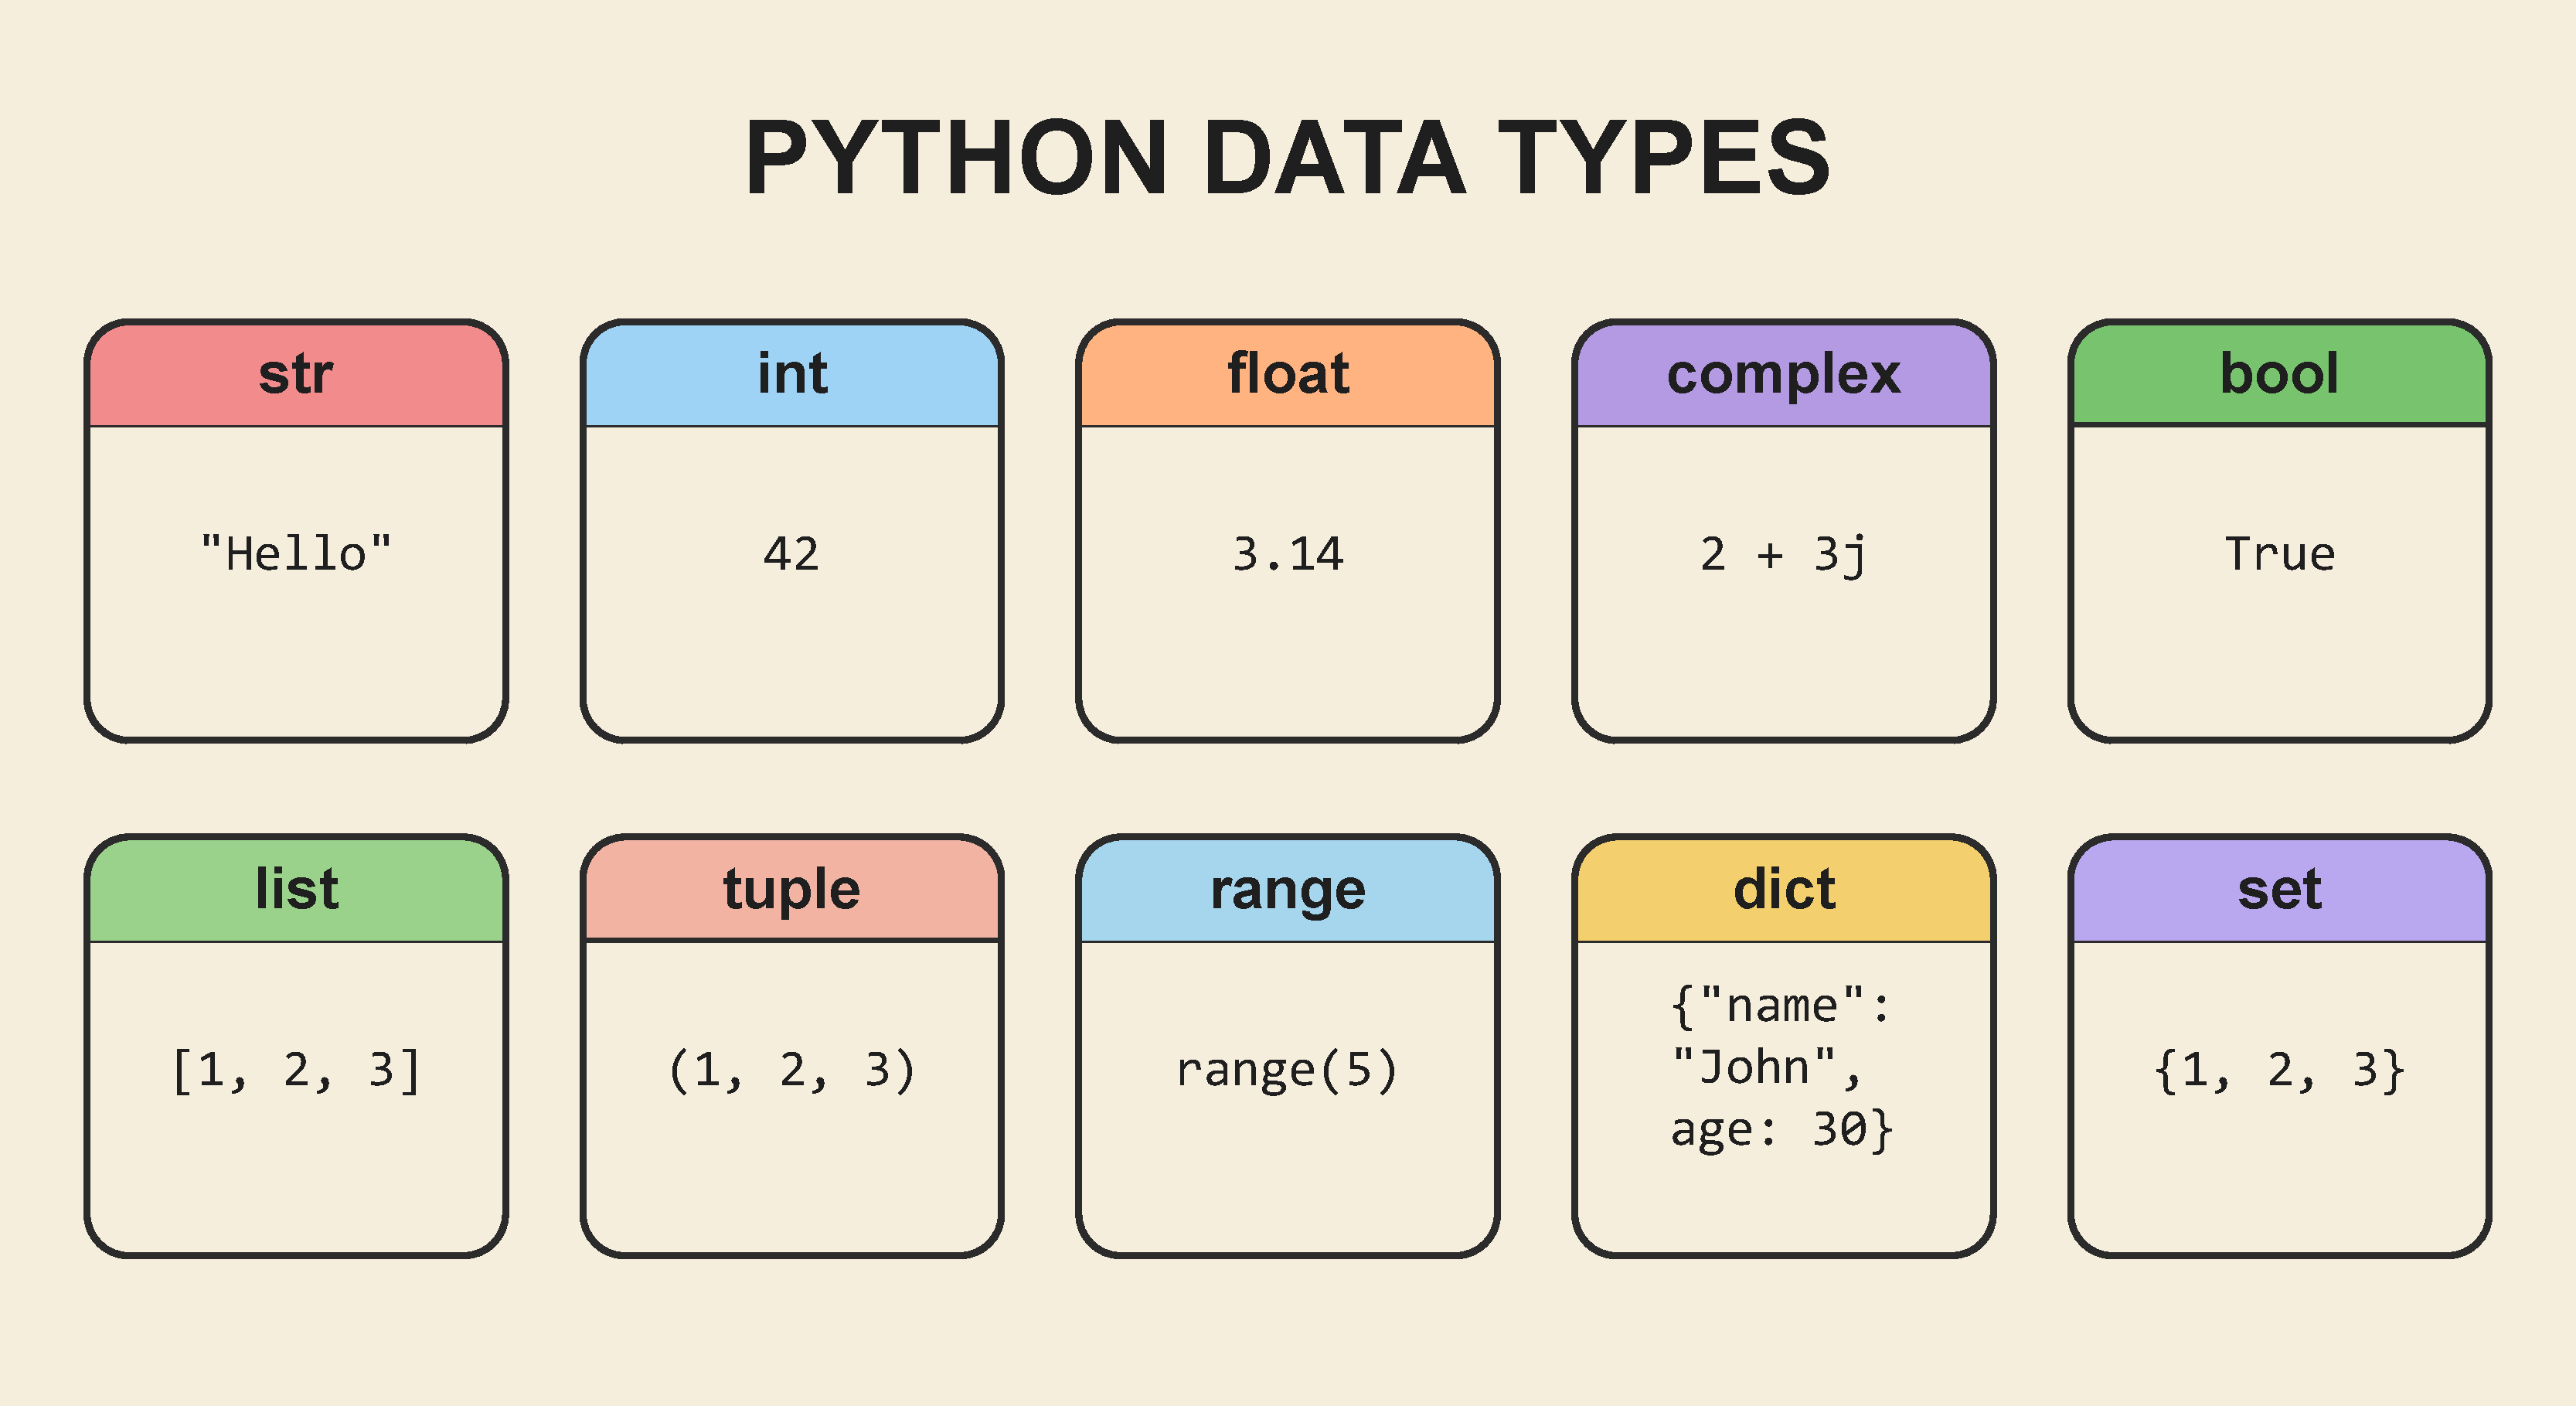
\includegraphics[width=\linewidth,keepaspectratio]{Figures/Data type/Fig_Data_type.pdf}
  \caption{Built-in Python data types grouped by category with simple literal examples.}
  \label{fig:py-dtypes}
\end{figure}
\medskip

\begin{tcolorbox}[% passing options here
    title=Focus of this chapter:,
    colframe=orange,
    colback = white,
%    colback=orange!40!yellow!30, % think of mixing 2 colors with sliders
    arc=2mm % sharp corners
 ]
\begin{itemize}
    \item Inspecting and converting types: Learn how to check what type a value has using \c{type(x)} or \c{isinstance(x, T)}, and how to convert safely (for example, \c{int("42")} when reading numbers from text input).
    \item Numeric types (\c{int}, \c{float}, \c{complex}, \c{bool}): Handle whole numbers, decimal values, engineering phasors, and logical values that behave like 1/0 in arithmetic.
    \item Text type (\c{str}): Work with human-readable labels, units, or codes, and format them with slicing, joining, or f-strings for clean reports.
    \item Sequence types (\c{list}, \c{tuple}, \c{range}): Organize data in order: editable collections, fixed records, and evenly-spaced sequences.
    \item Mapping type (\c{dict}): Store look-ups such as \c{"C25"} -> \c{25}, or \c{"Room101"} -> \c{18.5}. Dictionaries provide fast key--value access.
    \item Set types (\c{set}, \c{frozenset}): Deduplicate repeated items and check membership quickly with operations like union (\c{|}) or intersection (\c{\&}).
    \item Binary data (\c{bytes}, \c{bytearray}, \c{memoryview}): Understand how Python handles raw data from files or BIM exports.
    \item Mutability (can the value change?): Know which types can be edited in place (\c{list}, \c{dict}, \c{set}) versus which are fixed once created (\c{tuple}, \c{str}).
    \item Truthiness in conditions: See how Python decides if something counts as “empty/false” (e.g., \c{0}, \c{""}, \c{[]}) or “true” in an \c{if} or \c{while}.
    \item Choosing the right type and common pitfalls: Guidelines for picking the right type, plus avoiding traps such as mutable defaults (\c{def f(x, cache=\{\})}) or unhashable keys in \c{dict}.
\end{itemize}
\end{tcolorbox}
\hh{Inspecting and converting types}
How to find a value's type with \c{type()} and \c{isinstance()},
and when to convert text to numbers. Validate first, then convert; never assume user input is numeric.


\begin{itemize}
    \item Use \c{type(x)} to check the type of a value.
    \item Use \c{isinstance(x, T)} to test if \c{x} belongs to type \c{T} (or a subclass).
    \item Convert between types with constructors: \c{int("42")}, \c{float("3.5")}, \c{str(3.14)}, \c{list(iterable)}, \c{tuple(iterable)}, \c{set(iterable)}.
\end{itemize}

\code{c03_check_type}{python}{
    print(type(7))
    print(isinstance(True, int))   # bool behaves like a small integer
    floors = ["B1", "1", "2", "3"]
    print(type(floors))            # list
}{Quick type checks}

\hh{Memory Use of Data Types in Python}

In Python, a variable is more than just raw data. Every value is an \emph{object} with extra information attached.  
Think of it like a material delivery to a construction site: you don't just get the steel beam; you also get a tag, a shipping manifest, and packaging.  

Each object in Python carries:
\begin{itemize}
  \item \textbf{Object type}: what kind of data it is (integer, string, list, etc.).
  \item \textbf{Reference count}: how many variables are currently pointing to it (for memory management).
  \item \textbf{Size of the data}: the actual storage needed for the value.
\end{itemize}

Because of this overhead, even "simple" values use more memory than you might expect.  

\hhh{Memory Usage of Common Types}

\begin{itemize}
  \item \textbf{Boolean ({True}, {False})}  
  Fixed and small (about 28 bytes).  
  \emph{Analogy:} A light switch --- only on or off. Python creates the concept once, and variables just point to it.  

  \item \textbf{Integer ({int})}  
  Starts around 28 bytes for small numbers; grows as numbers get larger (Python integers are arbitrary precision).  
  \emph{Analogy:} A stack of bricks --- a small number is a small stack, a huge number is a tall stack.  

  \item \textbf{Float ({float})}  
  Usually a fixed size (about 24 bytes), represented as a C \c{double}.  
  \emph{Analogy:} A standard-sized window pane --- precise and pre-fabricated.  

  \item \textbf{String ({str})}  
  Overhead plus storage per character (about 49 bytes base + 1 byte/char in ASCII; more for Unicode).  
  \emph{Analogy:} A custom-length steel beam --- base cost plus extra material per unit length.  

  \item \textbf{List ({list})}  
  Overhead (about 64 bytes) plus pointers (8 bytes each on 64-bit systems). The list stores references, not the objects themselves.  
  \emph{Analogy:} A warehouse shelving unit --- the frame has size (overhead), but each slot points to where the items are stored.  

  \item \textbf{Dictionary ({dict})}  
  Large base overhead (about 240 bytes) since it is a hash table with spare capacity for efficiency. Memory grows with key--value pairs.  
  \emph{Analogy:} A building’s mailroom --- the board itself is big to leave room for new tenants, and each new mailbox adds more slots.
\end{itemize}
Figure \ref{fig:DATA-memory} summaries the membry use of data types in python.
\begin{figure}[htp!]
  \centering
  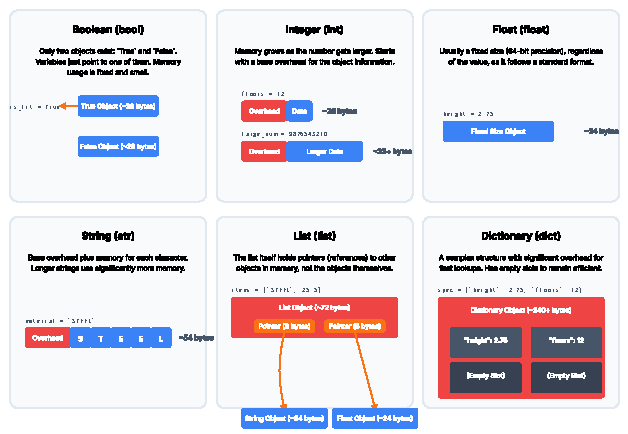
\includegraphics[width=\linewidth,keepaspectratio]{Figures/Data type/Memory usage.pdf}
  \caption{Memory use of data types in Python.}
  \label{fig:DATA-memory}
\end{figure}

\hhh{Checking Memory in Python}

You can measure approximate memory use with the \c{sys} module.  
Note that for collections, \c{getsizeof()} shows only the container’s size, not the total of all elements inside.

\code{c03_memory}{python}{
    import sys

    # Example data
    building_name = "Burj Khalifa"
    floors = 163
    height_meters = 829.8
    materials = ["steel", "concrete", "glass"]
    
    print(f"'{building_name}' (string) uses: {sys.getsizeof(building_name)} bytes")
    print(f"{floors} (integer) uses: {sys.getsizeof(floors)} bytes")
    print(f"{height_meters} (float) uses: {sys.getsizeof(height_meters)} bytes")
    print(f"The list itself uses: {sys.getsizeof(materials)} bytes")

    # Output (may vary by system):
    # 'Burj Khalifa' (string) uses: 61 bytes
    # 163 (integer) uses: 28 bytes
    # 829.8 (float) uses: 24 bytes
    # The list itself uses: 88 bytes
}{Measuring memory with {sys.getsizeof()}.}


\hh{Numeric types: int, float, complex, bool}
\c{int} represents whole numbers. \c{float} represents decimal numbers. \c{complex} numbers carry real and imaginary parts. \c{bool} represents \c{True} or \c{False} and acts like 1 or 0 in arithmetic.

\code{c03_numbers}{python}{
    span_m = 8.0        # float
    bays   = 5          # int
    beam_count = bays + 1
    tributary_width = span_m / 2    # true division

    panels_down = 7
    rows_needed = -panels_down // 3 # floor division
    print(beam_count, tributary_width, rows_needed)

    z = 2 + 3j
    print(z.real, z.imag)
}{Numeric types in action}

\textbf{Note.} Floats are fine for geometry. Use \c{decimal.Decimal} if you need exact currency or rational math.

\hh{Text: {str}}
Strings (\c{str}) are sequences of characters (Unicode) and are immutable. Common tasks: slicing, case changes, trimming, splitting, joining, and f-strings for formatting.

\code{c03_str}{python}{
    # Strings are 0-indexed; [:10] returns characters 0..9
    msg = "ARC Studio - North Wing"
    print(msg[:10]) # ARC Studio
    print(msg[4:10]) # Studio
    print(msg[-4:]) # Wing (last 4 characters)
}{Numeric types in action}

\hhh{Slicing substrings}

\code{c03_str_slicing}{python}{
    msg = "ARC Studio - North Wing"

    # Slices are 0-based; stop index is exclusive
    print(msg[:10])     # first 10 chars -> "ARC Studio" (0..9)
    print(msg[4:10])    # "Studio"       (4..9)
    print(msg[-4:])     # last 4 chars   -> "Wing"
    print(msg[0:3])     # "ARC"          (0,1,2)

    # Optional: step slicing (every 2nd character)
    print(msg[::2])
}{Extract parts of a string with slices}

\hhh{Case changes}

\code{c03_str_case}{python}{
    s = "concrete beam"
    print(s.upper())     # "CONCRETE BEAM"
    print(s.title())     # "Concrete Beam"
    print(s.lower())     # "concrete beam"
}{Upper/lower/title case}

\hhh{Trimming whitespace and simple unit cleanup}

\code{c03_str_trim}{python}{
    raw = "   GLT beam   \n"
    print(raw.strip())    # "GLT beam"  (trim both ends)
    print(raw.lstrip())   # "GLT beam   \n" (left only)
    print(raw.rstrip())   # "   GLT beam"   (right only)

    # Remove a trailing unit (simple case) before converting
    span_text = "9.25 m"
    span_m = float(span_text.replace(" m", ""))  # -> 9.25
    print(span_m)
}{Trim spaces and remove a simple trailing unit}

\hhh{Splitting into parts}

\code{c03_str_split}{python}{
    label = "Level 2 - East Wing"
    parts = label.split(" - ")
    print(parts)              # ["Level 2", "East Wing"]

    # Split CSV-like numbers and convert to floats
    dims_csv = "3.2,4.0,2.8"
    dims = [float(x) for x in dims_csv.split(",")]
    print(dims)               # [3.2, 4.0, 2.8]
}{Split by a delimiter (e.g., " - " or ",")}

\hhh{Joining pieces back together}

\code{c03_str_join}{python}{
    pieces = ["Studio A", "Ground Floor"]
    path = " / ".join(pieces)
    print(path)               # "Studio A / Ground Floor"

    lines = ["Room 101", "Room 102", "Room 103"]
    paragraph = "\n".join(lines)
    print(paragraph)
}{Join lists of strings with a chosen separator}

\hhh{f-strings for readable formatting}

\code{c03_str_fstrings}{python}{
    width_m  = 3.25
    length_m = 4.10
    area_m2  = width_m * length_m

    # Insert variables directly; format to 2 decimals
    print(f"Area = {area_m2:.2f} m\u00B2")  # \u00B2 is superscript 2

    bldg = "ARC Studio"
    wing  = "North"
    rooms = 12
    print(f"{bldg} - {wing} Wing has {rooms} rooms")

    # Optional: align columns (left text, right numbers)
    mat = "Concrete"
    load_kN = 125.7
    print(f"{mat:<10} | {load_kN:>8.1f} kN")
}{Insert variables and control numeric formatting with f-strings}

\hhh{Immutability: methods return a new string}

\code{c03_str_immutable}{python}{
    s  = "m^2"
    s2 = s.replace("^2", "\u00B2")  # returns a NEW string
    print(s2)   # m²
    print(s)    # m^2 (original unchanged)
}{String methods do not modify the original}

\hh{Sequence types: list, tuple, range}
When to choose a mutable list vs an immutable tuple,
and how \c{range} supports loops and indexing.

\c{list} is ordered and mutable. \c{tuple} is ordered and immutable. \c{range} represents arithmetic progressions.

\code{c03_seq}{python}{
    floors = ["B1", "1", "2", "3"]
    floors.append("4")

    grid_axes = tuple("ABCDEFG")

    spans = range(0, 30, 6)
    print(floors, grid_axes, list(spans))
}{Sequence basics}

List comprehensions are concise ways to build lists.

\code{c03_listcomp}{python}{
    bay_centers_m = [3.0, 9.0, 15.0, 21.0]
    trib_widths = [ (right - left)/2
                    for left, right in zip([0]+bay_centers_m, bay_centers_m+[24.0]) ]
    print(trib_widths)
}{Derived data with a list comprehension}

\hh{Mapping type: dict}

Fast key->value lookups for schedules and metadata.
Keys must be immutable; strings and tuples are common choices. Dictionaries (\c{dict}) map keys to values. Keys must be immutable and hashable.

\code{c03_dict}{python}{
    fc_MPa = {"C20": 20, "C25": 25, "C30": 30}
    steelFy_MPa = {("A36", "plate"): 250, ("A992", "shape"): 345}

    print(fc_MPa["C25"])
    print(steelFy_MPa[("A992", "shape")])
    print(fc_MPa.get("C40", "unknown grade"))
}{Dictionary lookups}

\code{c03_set_basics}{python}{
    materials = ["A992", "A992", "C30", "C30", "GLT"]
    unique = set(materials)                     # {'A992', 'C30', 'GLT'} (order not guaranteed)
    print(sorted(unique))                       # Outcome: ['A992', 'C30', 'GLT']

    print("A992" in unique)                     # Outcome: True
    print("A36"  not in unique)                 # Outcome: True

    # {} is a dict; use set() for an empty set
    empty_dict = {}
    empty_set  = set()
    print(type(empty_dict), type(empty_set))    # Outcome: <class 'dict'> <class 'set'>
}{Deduplication and membership}

\hhh{Add and remove items}
Add with \c{add} (single) or \c{update} (many). Remove with \c{remove} (errors if missing) or \c{discard} (silent if missing).

\code{c03_set_add_remove}{python}{
    s = {"concrete", "steel"}
    s.add("glass")
    print(sorted(s))                            # Outcome: ['concrete', 'glass', 'steel']

    s.update(["wood", "aluminum"])
    print(sorted(s))                            # Outcome: ['aluminum', 'concrete', 'glass', 'steel', 'wood']

    s.discard("copper")                         # ok even if not present
    print(sorted(s))                            # Outcome: ['aluminum', 'concrete', 'glass', 'steel', 'wood']

    # remove raises KeyError if the item is absent
    try:
        s.remove("copper")
    except KeyError as e:
        print("Missing:", e)                    # Outcome: Missing: 'copper'

    # pop removes and returns an arbitrary element
    taken = s.pop()
    print("popped:", taken)                     # Outcome: popped: (some element)
    print(len(s) >= 4)                          # Outcome: True
}{Adding/removing with add, update, discard, remove, pop}

\hhh{Set algebra: union, intersection, difference, symmetric difference}
Combine sets to answer “either”, “both”, “only in A”, and “in one but not both”.

\code{c03_set_ops}{python}{
    have = {"A992", "C30", "GLT"}
    want = {"A992", "A36", "GLT"}

    union  = have | want                        # either
    inter  = have & want                        # both
    diff   = have - want                        # only in have
    symdif = have ^ want                        # in one but not both

    print(sorted(union))                        # Outcome: ['A36', 'A992', 'C30', 'GLT']
    print(sorted(inter))                        # Outcome: ['A992', 'GLT']
    print(sorted(diff))                         # Outcome: ['C30']
    print(sorted(symdif))                       # Outcome: ['A36', 'C30']
}{Union, intersection, difference, symmetric difference}

\hhh{Subset, superset, and disjoint checks}
Express “is contained in”, “contains all of”, and “shares nothing with”.

\code{c03_set_relations}{python}{
    a = {"L1", "L2"}
    b = {"B1", "L1", "L2", "L3"}

    print(a <= b)                               # Outcome: True   (subset, allows equality)
    print(a <  b)                               # Outcome: True   (proper subset)
    print(b >= a)                               # Outcome: True   (superset)
    print(b.isdisjoint({"Roof"}))               # Outcome: True   (no common items)
}{Subset/superset ({<=}, {>=}) and disjointness}

\hh{Sets type}

\begin{NoteBox}
Both \c{set} and \c{dict} use curly braces \c{\{\}}, but they serve very different purposes.  
\begin{itemize}
    \item A \textbf{dictionary} (\c{dict}) maps \emph{keys} to \emph{values}, like a real dictionary (word $\to$ meaning).
    \item A \textbf{set} (\c{set}) holds only \emph{unique values}, with no duplicates and no key--value pairing.
\end{itemize}
\end{NoteBox}

\hhh{Dictionary ({dict})}
A dictionary stores key--value pairs. Each key must be unique and hashable (numbers, strings, tuples). Values can be of any type.

\code{c_dict}{python}{
    # Dictionary example
    building = {"rooms": 12, "floors": 3, "name": "ARC Studio"}
    print(building["rooms"])     # 12
    print(building["name"])      # ARC Studio
}{A dictionary maps keys to values}

\items{
¤ Syntax: \c{{"key": value, ...}}  
¤ Keys must be unique; values can repeat.  
¤ Empty dictionary: \c{{}}  
¤ Use when you want to \textbf{look up} values by a key.
}

\hhh{Set ({set})}
A set stores only values, and automatically removes duplicates. Useful for membership tests and mathematical set operations.

\code{c_set}{python}{
    # Set example
    materials = {"steel", "concrete", "glass", "steel"}
    print(materials)       # {'steel', 'glass', 'concrete'}
    print("glass" in materials)  # True
}{A set holds unique values}

\items{
¤ Syntax: \c{{value1, value2, ...}}  
¤ No key--value pairs; just values.  
¤ Empty set: \c{set()} (not \c{{}}).  
¤ No duplicates allowed.  
¤ Use for \textbf{unique collections} or set operations (union, intersection).
}

\hhh{Quick Comparison}

\begin{center}
\begin{tabular}{|l|c|c|}
\hline
 & \textbf{Dictionary ({dict})} & \textbf{Set ({set})} \\
\hline
Syntax & \c{{"key": value}} & \c{{value1, value2}} \\
Empty form & \c{{}} (empty dict) & \c{set()} (empty set) \\
Structure & Key $\to$ Value mapping & Unique values only \\
Duplicates & Keys unique, values can repeat & No duplicates at all \\
Use case & Lookup, mapping & Membership, uniqueness \\
\hline
\end{tabular}
\end{center}

\hh{Tuple type}
A tuple is an ordered, immutable sequence. Use it for fixed records like coordinates (x, y, z), room dimensions (width, length), or any small packet of values that should not change.

\hhh{Create and read tuples}
Define tuple literals, access items by index (0-based; negatives from the end), and build tuples from other iterables.

\code{c03_tuple_intro}{python}{
    # Coordinates (x, y, z) in meters
    node_A = (3.0, 0.0, 4.0)
    print(node_A)                   # Outcome: (3.0, 0.0, 4.0)
    print(node_A[0])                # Outcome: 3.0
    print(node_A[-1])               # Outcome: 4.0

    # Tuple from other iterables
    floors = tuple(["B1", "L1", "L2"])
    print(floors)                   # Outcome: ('B1', 'L1', 'L2')
}{Tuples are ordered sequences you cannot modify in place}

\hhh{Unpacking (assign many names at once)}
Unpacking lets you assign multiple variables in one step; the swap pattern (a, b = b, a) is a concise idiom.

\code{c03_tuple_unpack}{python}{
    dims = (3.2, 4.0)               # (width, length)
    w, l = dims                     # unpack into two variables
    print(w, l)                     # Outcome: 3.2 4.0

    # Swap values without a temp variable
    a, b = 10, 20
    a, b = b, a
    print(a, b)                     # Outcome: 20 10
}{Unpack tuples and swap values succinctly}

\hhh{Immutability (cannot change items)}
Tuples cannot be edited in place; to “change” a value, create a new tuple from pieces of the old one.

\code{c03_tuple_immutability}{python}{
    node = (2.5, 7.0)
    # node[0] = 3.0   # TypeError if you uncomment this line
    print(len(node))                # Outcome: 2

    # You can make a new tuple instead
    node = (3.0,) + node[1:]       # prepend 3.0 to the rest
    print(node)                     # Outcome: (3.0, 7.0)
}{Tuples don’t support item assignment; create a new tuple instead}

\hhh{Methods: count and index}
Tuples only expose a few sequence methods—most commonly count(value) and index(value).

\code{c03_tuple_methods}{python}{
    bays = (1, 2, 2, 3, 3, 3)
    print(bays.count(3))            # Outcome: 3   (three 3s)
    print(bays.index(2))            # Outcome: 1   (first 2 at index 1)
}{Tuples support count and index}

\hhh{Single-element tuples (mind the comma)}
A 1-tuple needs a trailing comma; parentheses alone do not make a tuple.

\code{c03_tuple_singleton}{python}{
    t1 = (5)                        # just an int in parentheses
    t2 = (5,)                       # a 1-tuple
    print(type(t1))                 # Outcome: <class 'int'>
    print(type(t2))                 # Outcome: <class 'tuple'>
}{Use a trailing comma for a 1-item tuple}

\hhh{Tuple vs list: when to use which}
Choose tuples for fixed, read-only records; choose lists for collections you plan to edit.

\code{c03_tuple_vs_list}{python}{
    dims_tuple = (3.2, 4.0)         # fixed (width, length) record
    dims_list  = [3.2, 4.0]         # will be edited later

    # Attempting to mutate the tuple will fail (TypeError if uncommented):
    # dims_tuple[0] = 3.0

    # Lists can be edited in place
    dims_list[0] = 3.0
    print(dims_tuple)               # Outcome: (3.2, 4.0)
    print(dims_list)                # Outcome: [3.0, 4.0]
}{Use tuples for fixed records; lists for editable collections}

\hhh{Conversions and iteration}
Convert between list and tuple as needed; iterate over a tuple just like any sequence.

\code{c03_tuple_convert_iter}{python}{
    areas_list = [12.0, 9.5, 16.2]
    areas_tuple = tuple(areas_list)
    print(areas_tuple)              # Outcome: (12.0, 9.5, 16.2)

    # Iterate like a list
    for a in areas_tuple:
        print(a)                    # Outcome: 12.0 \n 9.5 \n 16.2
}{Convert list<->tuple and iterate over tuples}

\hhh{Tuples as dictionary keys (hashable)}
Because tuples are immutable, they are hashable and can serve as keys in dictionaries.

\code{c03_tuple_as_key}{python}{
    # Use (x, y) coordinate as a key in a dict
    loads_kN = {
        (0, 0): 12.5,
        (0, 1): 15.0,
        (1, 0): 10.0
    }
    print(loads_kN[(0, 1)])         # Outcome: 15.0
}{Tuples can be keys because they are immutable (hashable)}

\hhh{Returning multiple values from a function}
Functions often return several results as a single tuple; unpack immediately for clarity.

\code{c03_tuple_return_swap}{python}{
    def room_stats(width, length):
        area = width * length
        perimeter = 2 * (width + length)
        return area, perimeter      # returns a tuple

    a, p = room_stats(3.0, 4.5)     # unpack results
    print(a, p)                     # Outcome: 13.5 15.0
}{Functions often return tuples; unpack them immediately}

\hhh{Caution: mutable items inside a tuple}
Tuple immutability is shallow: if a tuple holds a mutable object (like a list), that inner object can still change.

\code{c03_tuple_nested_mutable}{python}{
    # Tuple is immutable, but if it holds a mutable list, that list can change
    t = ( "grid", [0, 0] )
    t[1][0] = 9                     # modifying the inner list is allowed
    print(t)                        # Outcome: ('grid', [9, 0])
}{Tuple immutability is shallow; inner mutable objects can still change}

\hh{Range type}
A \c{range} represents an \emph{integer sequence} defined by \c{start}, \c{stop} (exclusive), and \c{step}.
It is {memory-efficient} (does not store all numbers) and is commonly used for loops, indexing, and simple integer grids.

\code{c03_range_intro}{python}{
    # stop-only: range(stop) -> 0, 1, 2, ..., stop-1
    r1 = range(5)                    # 0..4
    print(list(r1))                  # Outcome: [0, 1, 2, 3, 4]

    # start, stop: range(start, stop)
    r2 = range(2, 6)                 # 2..5
    print(list(r2))                  # Outcome: [2, 3, 4, 5]

    # start, stop, step: range(start, stop, step)
    r3 = range(0, 10, 2)             # even numbers < 10
    print(list(r3))                  # Outcome: [0, 2, 4, 6, 8]
}{Basic forms: stop-only; start--stop; start--stop--step}

\textbf{Stop is exclusive.} The last value is \c{stop - step} (not \c{stop}). Off-by-one mistakes often come from this.

\hhh{Common use: loops, labels, and grids}

\code{c03_range_loops}{python}{
    # Generate level labels: L1, L2, L3, L4
    levels = [f"L{n}" for n in range(1, 5)]
    print(levels)                    # Outcome: ['L1', 'L2', 'L3', 'L4']

    # Number bays across a span (e.g., 6 bays)
    for bay in range(1, 7):
        print(f"Bay {bay}")         # Outcome: Bay 1 ... Bay 6 (one per line)

    # Coordinate grid indices (rows x cols)
    rows, cols = 3, 4
    nodes = [(i, j) for i in range(rows) for j in range(cols)]
    print(nodes)                     # Outcome: [(0, 0), (0, 1), ..., (2, 3)]
}{Iterating with ranges: levels, bays, and grid indices}

\hhh{Length, membership, and indexing}

\code{c03_range_len_in}{python}{
    r = range(2, 11, 3)             # 2, 5, 8
    print(len(r))                   # Outcome: 3
    print(5 in r)                   # Outcome: True   (O(1) arithmetic check)
    print(7 in r)                   # Outcome: False

    # You can index a range (like a read-only sequence)
    print(r[0], r[1], r[-1])       # Outcome: 2 5 8

    # Slice a range; result is another range
    sub = r[0:2]                    # first two elements of r
    print(list(sub))                # Outcome: [2, 5]
}{Ranges support len(), membership tests, indexing, and slicing}

\hhh{Negative steps and descending sequences}

\code{c03_range_desc}{python}{
    # Descending floors: L5, L4, L3, L2
    for n in range(5, 1, -1):       # 5, 4, 3, 2
        print(f"L{n}")              # Outcome: L5, L4, L3, L2 (one per line)

    # Even grid lines descending
    evens_down = range(10, 0, -2)   # 10, 8, 6, 4, 2
    print(list(evens_down))         # Outcome: [10, 8, 6, 4, 2]
}{Use a negative step for descending sequences}

\textbf{Step must match direction.} If \c{start < stop}, use a positive \c{step}; if \c{start > stop}, use a negative \c{step}.  
\textbf{Step cannot be 0} (\c{ValueError}).

\hhh{Why range is memory-friendly}

\code{c03_range_memory}{python}{
    # Big iteration with small memory: range does not build a big list
    big = range(0, 1_000_000, 5)    # 0, 5, 10, ...
    print(big)                      # Outcome: range(0, 1000000, 5)
    print(big.start, big.stop, big.step)  # Outcome: 0 1000000 5

    # You can still take samples without materializing everything
    print(big[0], big[1], big[2])   # Outcome: 0 5 10
    print(len(big))                 # Outcome: 200000
}{Range stores only start/stop/step, not every element}

\textbf{Convert to list only when needed.} \c{list(range(...))} creates all elements in memory. Avoid this for huge ranges.

\hhh{Equality and sequence behavior}

\code{c03_range_equal}{python}{
    # Two ranges are equal if they represent the same sequence of integers
    print(range(0, 4, 2) == range(0, 5, 2))  # Outcome: False  ([0,2] vs [0,2,4])
    print(range(1, 4) == range(1, 5))        # Outcome: False

    # A range is not equal to a list, even if contents match
    print(range(3) == [0, 1, 2])             # Outcome: False  (different types)
}{Range equality compares sequences to other ranges only}

\hhh{Ranges are integer-only (what about floats?)}

\code{c03_range_floats}{python}{
    # range works with integers only:
    # range(0, 5, 0.5)  # TypeError

    # Simple float stepping: build a list yourself
    start, stop, step = 0.0, 2.0, 0.5
    vals = [start + i*step for i in range(int((stop - start)/step) + 1)]
    print(vals)                     # Outcome: [0.0, 0.5, 1.0, 1.5, 2.0]
}{Use a list comprehension for float steps (range is ints only)}

\hhh{Common pitfalls}

\code{c03_range_pitfalls}{python}{
    # 1) Off-by-one: stop is exclusive
    print(list(range(1, 4)))       # Outcome: [1, 2, 3] (not including 4)

    # 2) Direction mismatch
    print(list(range(5, 1, 1)))    # Outcome: []       (wrong direction with +step)
    print(list(range(5, 1, -1)))   # Outcome: [5, 4, 3, 2]

    # 3) Step cannot be zero
    try:
        bad = range(1, 5, 0)
    except ValueError as e:
        print("Error:", e)         # Outcome: Error: range() arg 3 must not be zero
}{Watch for exclusive stop, correct step sign, and step=0 errors}


\hh{Binary types}
\c{bytes}, \c{bytearray}, and \c{memoryview} represent raw data such as files. You will usually decode \c{bytes} to text with UTF-8.

\hh{Mutability quick guide}
\begin{itemize}
    \item Immutable: \c{int}, \c{float}, \c{complex}, \c{bool}, \c{str}, \c{tuple}, \c{frozenset}, \c{bytes}
    \item Mutable: \c{list}, \c{dict}, \c{set}, \c{bytearray}
\end{itemize}

\hh{Truthiness}
In conditions, Python treats \c{False}, \c{None}, zero, and empty collections as false; everything else is true. Test for None with \c{x is None}.

\code{c03_truth}{python}{
    rooms = []
    if rooms:
        print("has rooms")
    else:
        print("no rooms yet")

    width = 0.0
    if not width:
        print("width missing")

    x = None
    if x is None:
        print("no value assigned yet")
}{Truthiness examples}

\hh{Choosing the right type}
Quick heuristics: numbers for measures, strings for labels,
lists for editable sequences, tuples for fixed records, dicts for lookups, sets for uniqueness.


\begin{itemize}
    \item Ordered, editable items: \c{list}
    \item Fixed record or key: \c{tuple}
    \item Fast membership / deduplication: \c{set}
    \item Key to value lookup: \c{dict}
    \item Numeric math: \c{int} or \c{float}
    \item Text: \c{str}
    \item Binary I/O: \c{bytes} or \c{bytearray}
\end{itemize}

\hh{Mini practice}
\begin{enumerate}
    \item Floors = \c{["B1","1","2","2","3","3","3"]}. Produce a sorted list of unique floors.
    \item Build a dictionary mapping room name to area ($m^2$). Compute the average area, skipping \c{None} values.
\end{enumerate}

\hh{Common pitfalls}
\begin{itemize}
    \item Editing while iterating: avoid modifying a list during a loop.
    \item Mutable defaults: avoid \c{def f(x, cache=\{\})}. Use \c{None} and create inside.
    \item Hashability: never use \c{list} or \c{dict} as dictionary keys; use \c{tuple} or \c{str} instead.
\end{itemize}
